\chapter{Measures of Distribution} \label{ch:measuresdistribution}

Given the probability or probability density distribution of a random variable, a lot of information can be abstracted. For example, the expectation describes the average value of that random variable if the experiment is repeated many times.

Measures of distribution such as expectation and variance are introduced in this chapter.

\section{Expectation}

In probability and statistics sense, \textit{expectation} (also known as \textit{mean}) describes the average value of a random variable, if the variable is generated many times. For discrete random variable $X$, the expectation is given below.
\begin{eqnarray}
  \textup{E}(X) &=& \sum_{i=1}^{n}x_iP(x_i) \label{eq:expectationdiscrete}
\end{eqnarray}
where $\textup{E}(\cdot)$ is used to denote the expectation, and $n$ the cardinality of the sample space. For continuous random variable, it is
\begin{eqnarray}
  \textup{E}(X) &=& \int_{-\infty}^{\infty}xf(x)dx \label{eq:expectationcontinuous}
\end{eqnarray}
Expectation is sometimes denoted as $\mu$ in literatures.

Some features of expectation calculation are given below.
\begin{eqnarray}
  \textup{E}(cX) &=& c\textup{E}(X) \nonumber \\
  \textup{E}(X+Y) &=& \textup{E}(X) + \textup{E}(Y) \nonumber
\end{eqnarray}
where $c$ is a constant and $X$, $Y$ are two random variables. Furthermore, if $X$, $Y$ are independent,
\begin{eqnarray}
  \textup{E}(XY) &=& \textup{E}(X)\textup{E}(Y) \nonumber
\end{eqnarray}
These features can be easily derived from \eqref{eq:expectationdiscrete} and \eqref{eq:expectationcontinuous}.

\section{Variance and Standard Deviation}

Variance and standard deviation describe how spread samples are from its expectation. It is defined as follows.
\begin{eqnarray}
  \textup{Var}(X) &=& \textup{E}\left(\left(X-\textup{E}(X)\right)^2\right) \nonumber \\
  &=& \textup{E}\left(X^2-2X\textup{E}(X)+\textup{E}(X)^2\right) \nonumber \\
  &=& \textup{E}\left(X^2\right)-\textup{E}(X)^2 \label{eq:varderived} \\
  \sigma_X &=& \sqrt{\textup{Var}(X)} \nonumber
\end{eqnarray}
Variance and standard deviation are sometimes denoted as $\sigma^2$ and $\sigma$ respectively.

For zero-mean continuous random variables, from \eqref{eq:varderived} the variance is
\begin{eqnarray}
  \textup{Var}(X) &=& \int_{-\infty}^{\infty} x^2f(x)dx \nonumber 
\end{eqnarray}
This implies that for a non-bias estimation, the Mean Square Error (MSE) of the estimation is identical to the variance of the estimation. 

Some features of variance calculation are given below.
\begin{eqnarray}
  \textup{Var}(cX) &=& c^2\textup{Var}(X) \\
\end{eqnarray}
For independent random variables $X$ and $Y$,
\begin{eqnarray}
  \textup{Var}(X\pm Y) &=& \textup{Var}(X) + \textup{Var}(Y) \nonumber
\end{eqnarray}

Mean and standard deviation can be used to standardize a ransom variable as follows.
\begin{eqnarray}
  X^* &=& \dfrac{X-\mu}{\sigma} \nonumber
\end{eqnarray}
where $\mu$, $\sigma$ are the mean and standard deviation of random variable $X$ respectively. The standardized random variable, $X^*$, has a mean of $0$ and standard deviation of $1$.

\section{Moments}

In mathematics, the $r$-th moment of a continuous function $f(x)$ about $c$ is defined as follows.
\begin{eqnarray}
  \mu_n &=& \int_{-\infty}^{\infty}(x-c)^nf(x)dx \nonumber
\end{eqnarray}

By simply saying \textit{moment} without further explanation of $c$, it is by default that $c=0$. Let $f(x)$ be a PDF. In this sense, the $0$-th order and the $1$-st order moment of a probability density function can be calculated as follows.
\begin{eqnarray}
  && \mu_0 = \int_{-\infty}^{\infty}f(x)dx = 1 \nonumber \\
  && \mu_1 = \int_{-\infty}^{\infty}xf(x)dx = \textup{E}(X) \nonumber
\end{eqnarray} 
where it can be seen that the $0$-th and $1$-st moment of a PDF is 1 and its mean, respectively.

Further more, let $c=\mu_1$ be the mean of the random variable to calculate the second \textit{central moment} $\mu_2$ as follows.
\begin{eqnarray}
  \mu_2 = \int_{-\infty}^{\infty}(x-\mu_1)^2f(x)dx = \textup{Var}(X) \nonumber
\end{eqnarray} 
which is the variance of the random variable.

Using mean and variance to further define \textit{standardized moments} as follows. For $k\geq 3$,
\begin{eqnarray}
  && \bar{\mu}_k = \dfrac{\mu_k}{\sigma^k} \nonumber \\
  && \mu_k = \textup{E}\left((X-\mu)\right) = \int_{-\infty}^{\infty}(x-\mu)^kf(x)dx \nonumber \\
  && \sigma^k = \left(\mu_2\right)^{\dfrac{k}{2}} = \left(\int_{-\infty}^{\infty}(x-\mu)^2f(x)dx\right)^{\dfrac{k}{2}} \nonumber
\end{eqnarray}
where $\mu_1$ and $\mu_2$ are the aforementioned mean ($1$-st order moment) and variance ($2$-nd order central moment) of the random variable, respectively.

The $3$-rd and $4$-th order standardized moments are known as the \textit{skewness} and \textit{kurtosis} of the PDF, respectively, as shown below.
\begin{eqnarray}
  && \bar{\mu_3} \equiv \gamma_1 = \dfrac{\textup{E}(x-\mu)^3}{\sigma^3} \nonumber \\
  && \bar{\mu_4} \equiv \gamma_2 = \dfrac{\textup{E}(x-\mu)^4}{\sigma^4} \nonumber
\end{eqnarray}
where $\mu=\mu_1$ and $\sigma = \sqrt{\mu_2}$ are the mean and standard deviation of the random variable, respectively. 

The skewness $\gamma_1$ is a measure of asymmetry of the PDF. When $\gamma_1 > 0$ or positive skew, the distribution has a long tail on the right side of the PDF. When $\gamma_1 <0$ or negative skew, the distribution has a long tail on the left side. When $\gamma_1 = 0$, the PDF might be symmetric (but not necessarily so). Examples are given in Fig. \ref{fig:skewness_demo}.
\begin{figure}
	\centering
	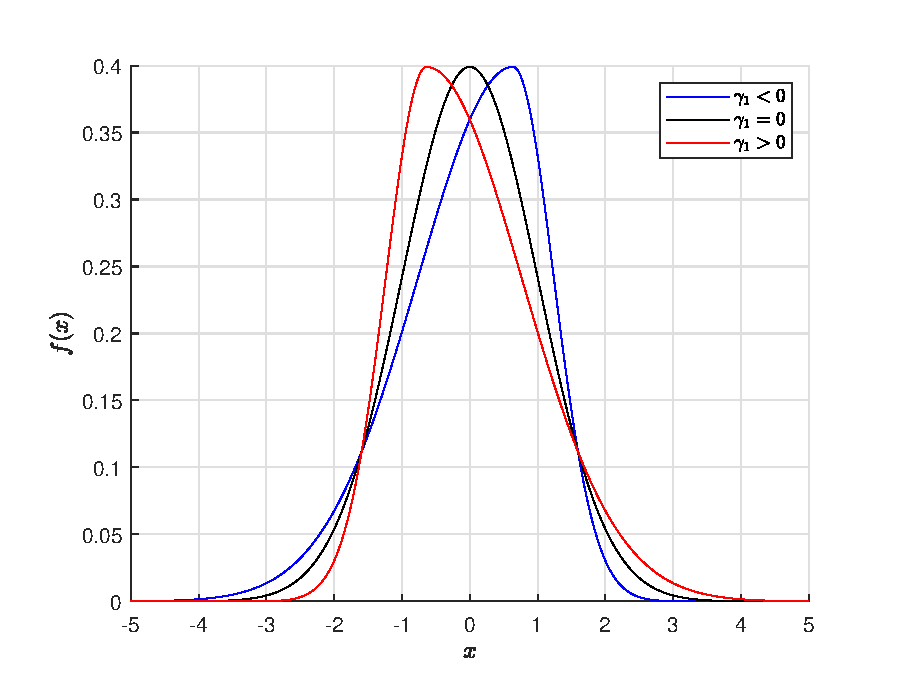
\includegraphics[width=250pt]{chapters/ch-measures-of-distribution/figures/skewness_demo.eps}
	\caption{Demonstration of PDF with different skewness.} \label{fig:skewness_demo}
\end{figure}

The kurtosis $\gamma_2$ measures the ``tailedness'' of a probability distribution, i.e., whether the PDF has heavy tail or thin tail. However, the kurtosis defined by the fourth standardized moment is often adjusted by subtracting 3 (which is the kurtosis of a standard normal distribution) to make it zero for a normal distribution.


\section{Correlation}


\section{Important Rules}


